\subsection{Speech Synthesis \cite{Jurafsky2006}}

This section is a summary of Chapter 8, Speech Synthesis of the book Speech and Language Processing \cite{Jurafsky2006}. In this summary we will see some main challenges and classic approaches of the \emph{text-to-speech (TTS)} task.

\begin{figure}[htbp]
  \centering
  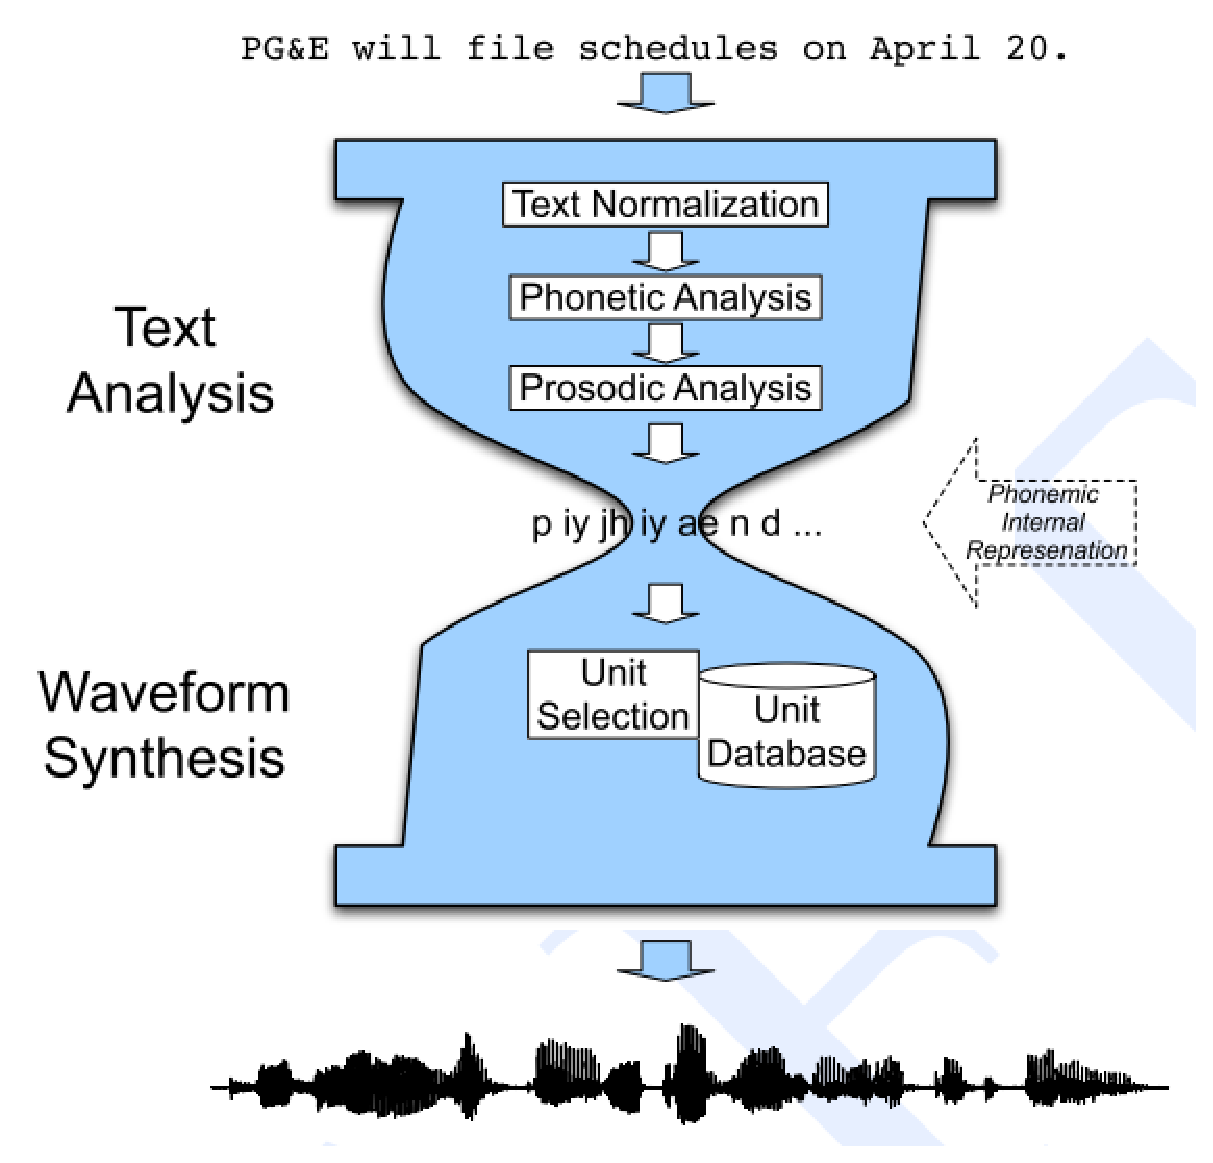
\includegraphics[width=.5\linewidth]{10_17_tts_arch}\\
  \caption{Architecture for the classic TTS system}\label{fig:TTS_arch}
\end{figure}

The goal of TTS is to map a text to a waveform output. The classic TTS architectures have two main steps, text analysis and waveform synthesis, as shown in Figure \ref{fig:TTS_arch}. While text analysis algorithms are relatively standard, there are three different paradigms for waveform synthesis: concatentative synthesis, formant synthesis and articulatory synthesis. Most modern commercial TTS systems are based on concatentative synthesis. Next we will explore each of the sub-tasks in further details.

The text analysis step has three main components: the text normalization component, the phonetic analysis component, and the prosodic analysis component. Each of them performs the following sub-tasks:
\begin{enumerate}
\item{Text Normalization:
    \begin{itemize}
    \item Sentence tokenization: This step segments a paragraph into a set of sentences, so that the TTS can synthesis speech for each sentence separately.
    \item Process non-standard words: There are several types of non-standard words, including numbers, abbreviations, acronyms and so on. For example, in `The European economy in 1750', the number 1750 is translated to `seventeen fifty'. But in `The password is 1750', the number should be translated to `one seven five zero'.
    \item Homograph disambiguation: Some words with the same spelling may have different pronunciations. For example, the word live in `live in China' should be pronounced differently from that in `a live animal'.
    \end{itemize}
}
\item{Phonetic Analysis: This stage takes the normalized word strings and produces a pronunciation for each word.
    \begin{itemize}
    \item Dictionary lookup: The first step is to directly lookup each word in the phonetic dictionary. For example, a sample entry in the CMU Pronouncing Dictionary is ``TABLE - T EY1 B AH0 L'' (0 denotes unstressed, 1 denotes stressed).
    \item Process names: There are many types of names, such as names of people, locations, organisations, etc. Some of the names may not appear in the dictionary. In the step the system need to decide how to pronounce them.
    \item Grapheme-to-phoneme: In this stage, the system uses letter-to-sound rules to process the remaining words.
    \end{itemize}
}
\item{Prosodic Analysis: The goal of the prosody analysis stage is to decide the rhythm, accent, stress, tune and other aspects of the speech.
    \begin{itemize}
    \item Prosodic structure: For example in a single phrase `I wanted to go to London', there seems to be some prosodic phrase boundaries that split up the words as follows: `I wanted | to go | to London'.
    \item Prosodic prominence: In any spoken utterance, some words sound more prominent than others. The notion of prominence is generally captured by a marker called pitch accent. The following example shows accented words in capital letters: `I'm a little SURPRISED to hear it.'
    \item Tune: A very obvious example of tune in English is the difference between statements and yes-no question. Consider the statement `you know what I mean' and the question `you know what I mean?'.
    \item Compute duration and F0 from prosodic labels: F0 refers to the lowest frequency of a complex wave. Some algorithms such as the unit selection synthesis approach do not need this step.
    \end{itemize}
}
\end{enumerate}

\begin{figure}[htbp]
  \centering
  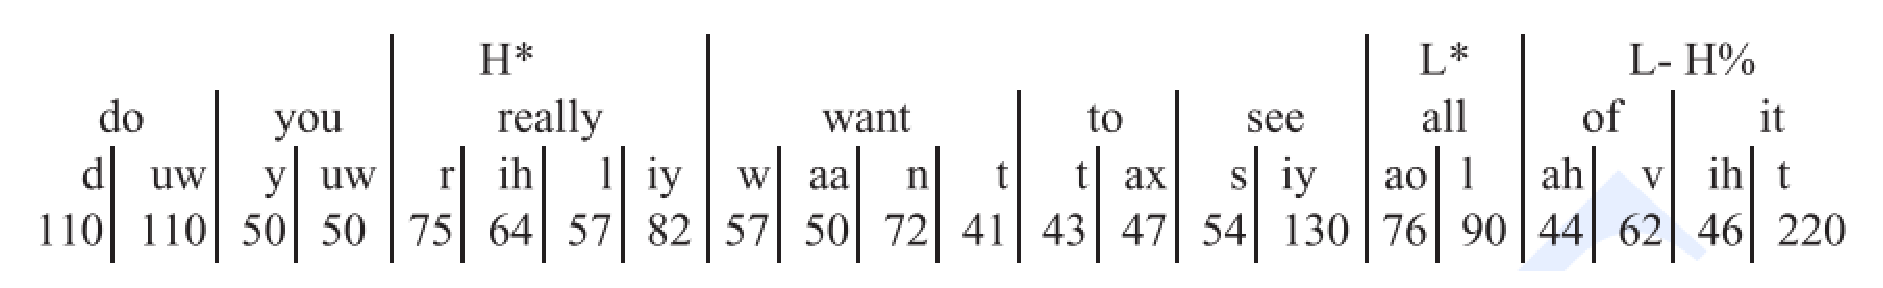
\includegraphics[width=.7\linewidth]{10_17_tts1}\\
  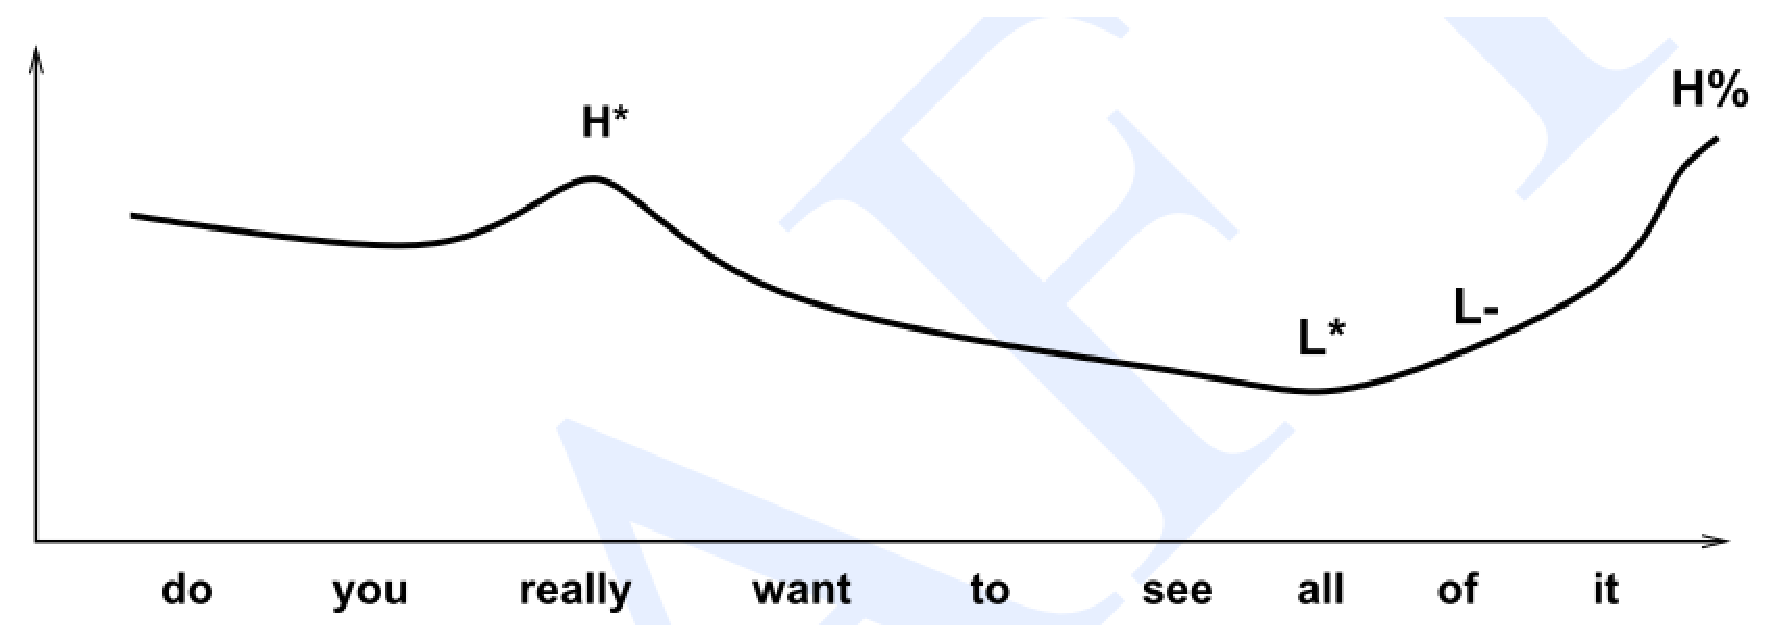
\includegraphics[width=.5\linewidth]{10_17_tts2}\\
  \caption{Internal representation of the FESTIVAL diphone system}\label{fig:TTS_inter}
\end{figure}

The final output of text analysis is called the internal representation of the input text sentence. Figure \ref{fig:TTS_inter} shows some TTS output from the FESTIVAL diphone system for the sentence `Do you really want to see all of it?'.

The next step is to turn the internal representation into a waveform. As aforementioned most of the modern commercial TTS systems are based on concatentative synthesis. The basic idea of concatentative approaches is to store the speech of human speakers in a database, and then retrieve and concatenate them according to the internal output. Two concatentative methods are discussed in this chapter: diphone synthesis and unit selection synthesis.

A diphone is a phone-like unit going from roughly the middle of one phone to the middle of the following phone. It takes a sequence of diphones from the database that corresponds to the desired phone sequence, and then concatenates them with some slight signal processing. Finally the algorithm performs some prosodic adjustments to the concatenated utterance.

Modern commercial TTS systems are based on a generalization of diphone synthesis, called unit selection synthesis. It differs from the classic diphone approach is two ways: 1) The unit selection database is much bigger (many hours long), containing many copies of each diphone; 2) Unit selection synthesis use no signal processing to the concatenated units, such as prosodic adjustments.

Finally, the section discusses some evaluation methods of the TTS systems. The development of a good automatic metric for speech synthesis remains an open question. Currently the speech synthesis systems are still evaluated by human listeners.

Remark: I think the TTS can be treated as an isolated component in our chatbot system. While it is intuitively beneficial to combine ASR and the dialogue manager (such as by jointly training), it seems difficult to improve TTS in a similar manner. I think we can use existing TTS system as a black box, without too much caring about how it works. 